
\documentclass[11pt]{article}
\usepackage{setspace}
\usepackage{amssymb, natbib}
\usepackage[tbtags]{amsmath}
\usepackage{rotating}
\usepackage{ctable}
\usepackage{sectsty}
\usepackage{fancyhdr}
\usepackage{caption}
\usepackage{comment}
\usepackage{appendix}
\usepackage{color}
\usepackage[bottom=1.16in]{geometry}
\usepackage{multirow} 	
\usepackage{lscape}

\usepackage[, pdftitle={QualQuan}, pdfauthor={HJ},
			hyperfootnotes=true, linkbordercolor={1 .9 .2}, citebordercolor={.2 .9 .5},
			urlbordercolor={.1 .9 1}]{hyperref}


\usepackage{array}
\newcolumntype{x}[1]
	{>{\raggedright}p{#1}}
\newcommand{\tn}{\tabularnewline}


%\usepackage{hypernat}

\newcommand{\revertstretch}{\setstretch{1.3}}
\revertstretch







% THEOREM Environments ---------------------------------------------------
 \newtheorem{thm}{Theorem}%[subsection]
 \newtheorem{cor}[thm]{Corollary}
 \newtheorem{lem}[thm]{Lemma}
 \newtheorem{thma}{Theorem}%[subsection]
 \newtheorem{lema}[thm]{Lemma}
 \newtheorem{prop}[thm]{Proposition}
% \theoremcontact{definition}
 \newtheorem{defn}[thm]{Definition}
% \theoremcontact{remark}
 \newtheorem{rem}[thm]{Remark}
 \newtheorem{hypo}{Hypothesis}
% \numberwithin{equation}{subsection} % MATH ------------------------------------------------------------------- %
\DeclareMathOperator{\IM}{Im} % \DeclareMathOperator{\ess}{ess}
 \newcommand{\eps}{\varepsilon}
 \newcommand{\fn}{\footnote}
 \newcommand{\To}{\longrightarrow}
 \newcommand{\h}{\mathcal{H}}
 \newcommand{\s}{\mathcal{S}}
 \newcommand{\A}{\mathcal{A}}
 \newcommand{\J}{\mathcal{J}}
 \newcommand{\M}{\mathcal{M}}
 \newcommand{\W}{\mathcal{W}}
 \newcommand{\X}{\mathcal{X}}
 \newcommand{\BOP}{\mathbf{B}}
 \newcommand{\BH}{\mathbf{B}(\mathcal{H})}
 \newcommand{\KH}{\mathcal{K}(\mathcal{H})}
 \newcommand{\Real}{\mathbb{R}}
 \newcommand{\Complex}{\mathbb{C}}
 \newcommand{\Field}{\mathbb{F}}
 \newcommand{\RPlus}{\Real^{+}}
 \newcommand{\Polar}{\mathcal{P}_{\s}}
 \newcommand{\Poly}{\mathcal{P}(E)}
 \newcommand{\EssD}{\mathcal{D}}
 \newcommand{\Lom}{\mathcal{L}}
 \newcommand{\States}{\mathcal{T}}
 \newcommand{\abs}[1]{\left\vert#1\right\vert}
 \newcommand{\set}[1]{\left\{#1\right\}}
 \newcommand{\seq}[1]{\left<#1\right>}
 \newcommand{\norm}[1]{\left\Vert#1\right\Vert}
 \newcommand{\essnorm}[1]{\norm{#1}_{\ess}}
%%% ----------------------------------------------------------------------
\newenvironment{changemargin}[2]{%
 \begin{list}{}{%
  \setlength{\topsep}{0pt}%
  \setlength{\leftmargin}{#1}%
  \setlength{\rightmargin}{#2}%
  \setlength{\listparindent}{\parindent}%
  \setlength{\itemindent}{\parindent}%
  \setlength{\parsep}{\parskip}%
 }%
\item[]}{\end{list}}



\color{black}
\title{Notes on Qualitative Inference}
\color{black}
\author{{\bf CU Senior Hons}}
\date{\today}


\begin{document}
\color{black}
\singlespacing
\maketitle

\thispagestyle{empty}

\section{What is qualitative analysis?}
It's surprisingly hard to pinpont what the analytic difference between qualitative and quantitative approaches is.
\begin{itemize}
	\item Number of cases?
	\item Use of numbers?
	\item Exploratory/inductive versus deductive?
	\item Interest in case effects versus general effects?
	\item Interest in what caused Y versus what's the effect of X?
	\item Subjective versus Objective?
	\item Descriptive versus Causal?
	\item Different notions of causality -- INUS, equifinality, necessity and sufficiency? Deterministic versus stochastic?
	\item Difference in data sources, eg direct observation, interviews, archives?
	\item A difference in general orientation? 	
	\item Something else? What?
\end{itemize}

 \newpage
\section{Causal inference for qualitative studies}

\subsection{The problem of causal inference}

Consider, to begin, a situation in which some individuals in a diseased population are observed to have received a treatment while others have not ($X$). Assume that, subsequently, a researcher observes which individuals become healthy and which do not ($Y$). Let us further assume that each individual belongs to one of four unobserved ``types,'' defined by the potential effect of treatment on the individual:

\begin{itemize}
    \item \textbf{a}dverse: Those who would get better if and only if they do not receive the treatment
    \item \textbf{b}eneficial: Those who would get better if and only if they do receive the treatment
    \item \textbf{c}hronic: Those who will remain sick whether or not they receive treatment
    \item \textbf{d}estined: Those who will get better whether or not they receive treatment
\end{itemize}

Throughout, we will use the letters $a,b,c,$ and $d$ to denote these causal types and the terms, $\lambda_a,\lambda_b,\lambda_c,\lambda_d$, to denote the relative share of these types in the population. 

These types differ in their ``potential outcomes'' | that is on what outcomes, $Y$,  they \textit{would} take on under alternative treatment conditions, $X$. More formally, we let $Y(x)$ denote a case or type's potential outcome  when $X=x$. Thus, the potential outcomes are $Y(0)=1, Y(1)=0$ for type $a$; $Y(0)=0, Y(1)=1$ for type $b$; $Y(0)=0, Y(1)=0$ for type $c$; and $Y(0)=1, Y(1)=1$ for type $d$.  These potential outcomes are illustrated in Table \ref{tabPO}.


\begin{table}[h!]
\begin{tabular}{l|cccc} \small

& Type a & Type b & Type c & Type d \\

& \textbf{a}dverse effects & \textbf{b}eneficial Effects & \textbf{c}hronic cases & \textbf{d}estined cases \\
\hline
Not treated &    Healthy &       Sick &       Sick &    Healthy \\
Treated &       Sick &    Healthy &       Sick &    Healthy \\
\end{tabular}  
\caption{Potential Outcomes: What would happen to each of four possible types of case if they were or were not treated.}
\label{tabPO}
\end{table}


\subsection{What we know and what we do not know}

The treatment effect for a case is defined as the difference in potential outcomes for that case between the treatment and control conditions, $Y(1)-Y(0)$. The \textit{fundamental problem of causal inference} is that, for any given case, it is only possible to observe $Y(1)$ or $Y(0)$. Thus, for no case is it possible to observe the difference between these two quantities and, hence, the treatment effect. Put differently, it is impossible to directly observe the \textit{type} of an individual case. 

Table \ref{FP} displays the ambiguity that we face about the type of a case given an observation of $X$ and $Y$ for that case.

\begin{table}[h!]
\centering
\begin{tabular}{c|cc}
           &        $Y=0$ &        $Y=1$ \\ \hline
       $X=0$ &     $b$ or $c$ &     $a$ or $d$ \\
       $X=1$ &     $a$ or $c$ &     $b$ or $d$ \\
\end{tabular}  
\caption{The fundamental problem of type ambiguity}
\label{FP} 
\end{table}


The key thing to note is that we know (or can measure) the value of $X$ and the value of $Y$. That means that we know which cell we are in. But we still do not know the \textit{type}. 


\section{A Qualitative Strategy for Causal Inference}
\subsection{Strategy}
The key strategy in process tracing is to look for ``clues'' that are indicative of the causal type. These clues are sometimes just called ``observable implications'' (especially when they come from a theory) or \textbf{CPOs}: Causal Process Observations (as distinct from DSOs -- Data Set Observations). Note that clues may be indicative of the causal type but you may also have clues that are indicative of more complex propositions, such as the presence of a given mechanism etc.

A clue has \textit{probative power} to distinguish between two hypotheses (say) when the probability of observing the clue is different under the two hypotheses.

Formally (or intuitively) you update given the clue using Bayes's rule which says:
\begin{eqnarray}
\Pr(H|\mathcal{D})=\frac{\Pr(\mathcal{D}|H)\Pr(H)}{\Pr(\mathcal{D})}
\end{eqnarray}

This means that the probability of the Hypothesis given the data is a function of: the prior probability of the hypothesis times the probability of seeing the data if the hypothesis is true, divided by the total probability of seeing the data.

\textbf{An example of Bayes rule: }I am interested in whether a coin is a fair coin (which comes up heads or tails with equal probability) or a biased coin (which comes up heads with a 2/3 probability). I think these two are equally likely. I toss the coin twice and it comes up heads twice! What should I infer about the probability that it is a fair coin?\footnote{
\rotatebox[origin=c]{180}{%
\noindent
\begin{minipage}[t]{\linewidth}
\textbf{Answer:} $\frac{\frac{1}{4} \times \frac{1}{2}}{  \frac{1}{4} \times \frac{1}{2} + \frac{4}{9}*\frac{1}{2}} = 9/25 = 0.36$
\end{minipage}
}
}
  
In this case observing the two heads is a clue (really just data) and you want to use it to draw inferences. 

The inferences you can draw from any clue depend hugely on how likely  you are to observe the clue under different conditions. Different combinations of probabilities give rise to four different types of qualitative ``tests'' (tests in quotes because this logic is useful even if you are not actually testing): the \textit{hoop test}, the \textit{smoking gun} test, the \textit{straw in the wind} test, and the \textit{doubly decisive} test. 

These tests and the kinds of inferences you can make from them are illustrated in the next two figures.

\begin{figure}[h!]
\centering
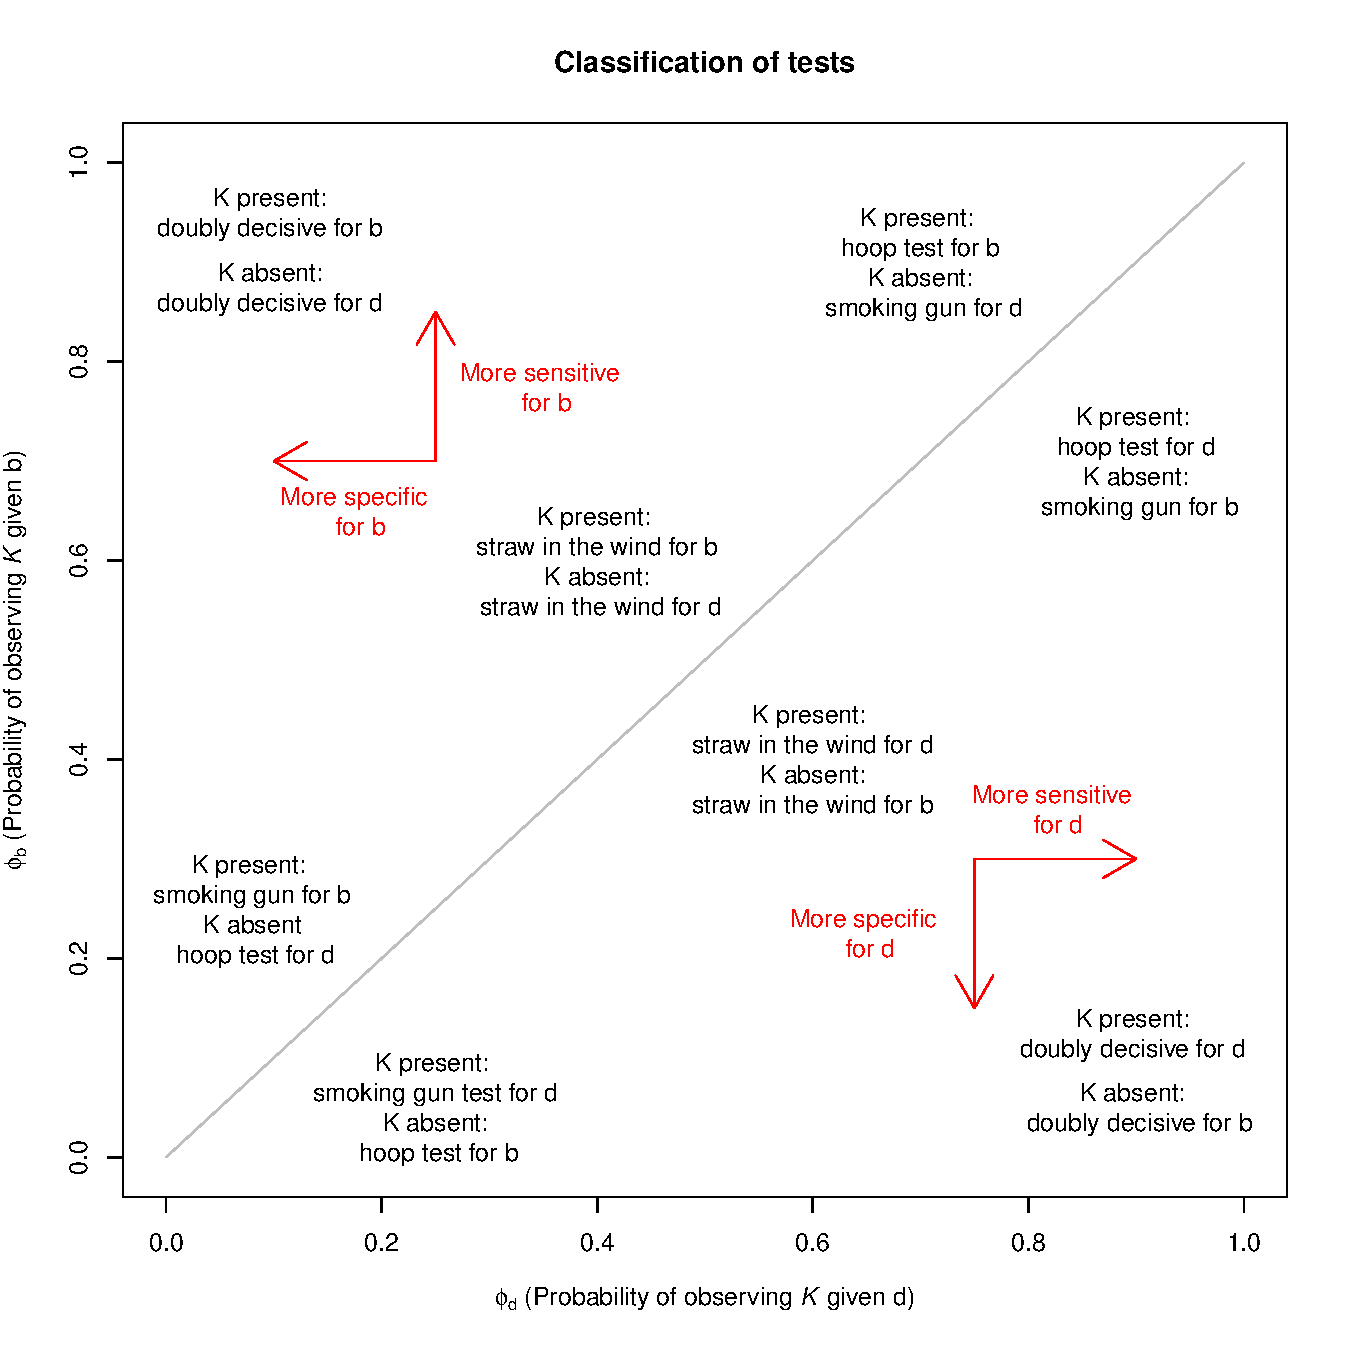
\includegraphics[width=\textwidth]{Figs/PTtests1.pdf}
\caption{{A mapping from the probability of observing a clue if a proposition "$b$"   to a generalization of the classic qualitative tests. }}
\label{CluesInferences1}
\end{figure}


\begin{figure}[h!]
\centering
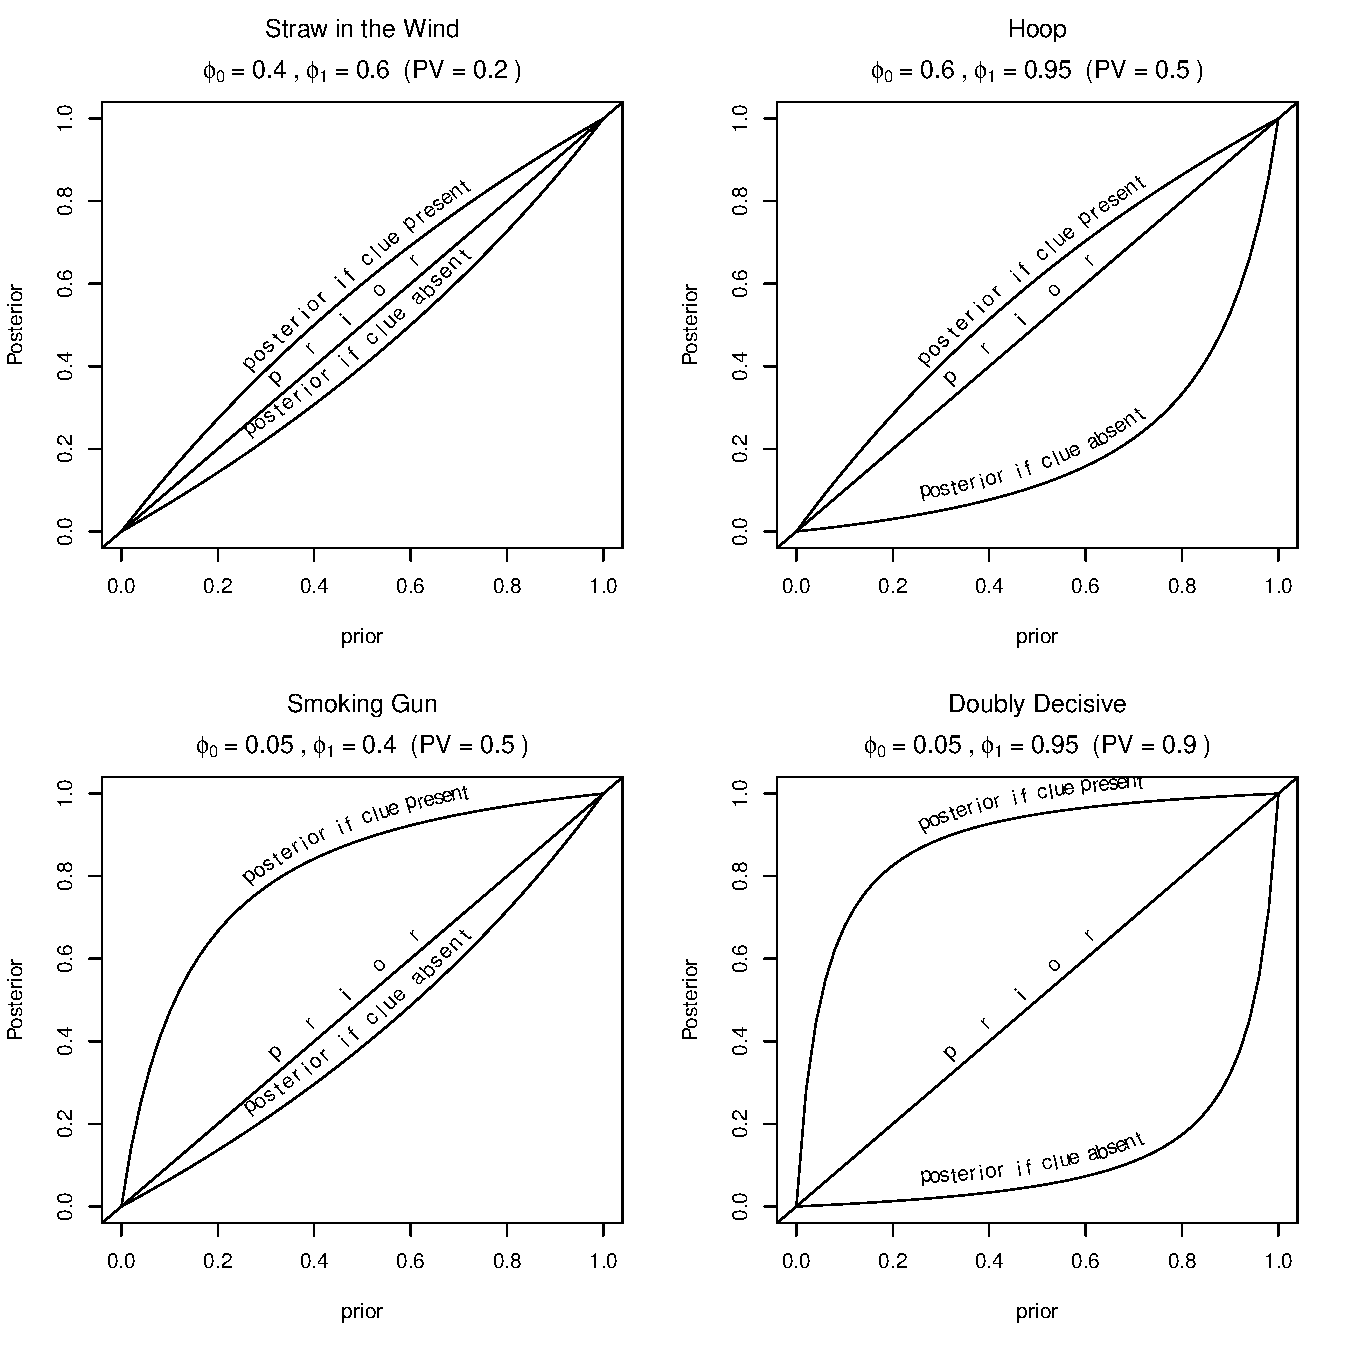
\includegraphics[width=.8\textwidth]{Figs/PTtests2.pdf}
\caption{\small{Figure shows how the learning from different types of tests depends on priors regarding the proposition. A ``smoking gun'' test has the greatest impact on beliefs when priors are middling low and the clue is observed; a ``hoop test'' has the greatest effect when priors are middling high and the clue is not observed. Here ``PV'' denotes the probative value of the test.}}
\label{CluesInferences2}
\end{figure}



\subsection{Questions}
Make sure you can answer all these questions:
\begin{enumerate}
\item	Say you look at a case with $X=1$ and $Y=1$: what is this unit's causal type?
\item	Say you look at a case with $X=1$ and $Y=0$: what is this unit's causal type?
\item	Give an example of a smoking gun test
\item   Explain how you know that this is a smoking gun test
\item	Give an example of a hoop test
\item   Explain how you know that this is a hoop test
 
\end{enumerate}

 \newpage

\section{In-class Exercise}

Here are the same four arguments from yesterday. For each argument you should:
\begin{enumerate}
\item identify the \textbf{overall causal relationship }of interest
\item propose a smoking gun OR a hoop test for the relationship
\item give an argument for why it is a smoking gun (or hoop) test
\item identify a key  \textbf{mechanism} of interest (or, better, pair of rival mechanisms)
\item propose a smoking gun OR a hoop test for the mechanism
\item give an argument for why it is a smoking gun (or hoop) test
\item describe what sort of case would be the best one to choose in order to assess the overall causal relationship (eg $X = 1$, $Y = 1$)? 
\end{enumerate}
\small
\subsection{Natural resources and conflict}
In developing countries that discover natural resources, such as oil, the ruling elite can extract wealth without needing to tax citizens and develop the state apparatus. Because the state does not rely on taxation for government revenue, it does not need to set up accountability structures or extend its reach and citizens do not feel that they have ownership over the state. The state therefore becomes both less democratic and weaker than if it had not discovered the resources.

\subsection{Democracy and growth}
Rich countries are more likely to be democratic for the simple reason that when people become wealthier they refuse to be dictated to by others and they demand a role in government. The marginal effects of income increases are greater for poorer countries because the impacts on eduction are greatest at these levels. You can test this proposition by exploiting natural variation in commodity prices which provide shocks to national income, especially for countries dependent on primary commodity exports.

\subsection{Factor Endowments and Coalitions}
When countries increase trade (imports and exports), the returns to economic factors (such as labor, land and capital) are affected differently. Specifically, the returns to factors that are the most \textit{abundant} are positive, while the returns to factors that are the most \textit{scarce} are  negative. Therefore, the relative factor endowments of a country will predict what sort of political coalitions will form (eg Land versus Labor + Capital) and which groups will favor free trade policies. 

\subsection{Democratic peace}
In democratic states, leaders are accountable for any losses incurred as a result of the wars that they enter into. Two states with democratic leaders are also more likely to share a common set of norms, and to engage in trade with one another. Therefore, two democracies are far less likely to enter into war with one another than a democracy and a non-democracy, or two non-democracies.
\newpage
\section{Case selection}
\subsection{Selection on the dependent variable}
eg to understand why there are revolutions you have to look at those cases with revolutions. Concern though is that you may be wrong thinking that X is a cause of Y if X is also present in those cases where Y is not. More generally censoring on Y can lead to bias. When might it make sense?

\subsection{Random case selection}
What advantages and disadvantages?

\subsection{Typical cases?}
Typical of model or typical of data? Say X = (1, 2, 3, 100), Y = c(1,2,3,0). What case is typical?

\subsection{Diverse cases?}
To represent the  distribution of the support of the data?

\subsection{Extreme cases?}
Extreme in terms of data, Hard cases and bad laws?

\subsection{Deviant cases?}
Extreme in terms of model error. Hard cases and bad laws?

\subsection{Influential?}
Is this really deviant?

\subsection{Most similar? Most Different}
Similar \textbf{except} on var of interest. 
Different \textbf{except} on vars of interest. 


\bigskip \\

\noindent \textbf{Question:} What is the implicit inference strategy? What do you \textit{do} with the cases?

\subsection{Easy cases? Hard cases?}
Sometimes people describe choosing ``most likely'' and ``least likely'' cases. For the intuition consider the claim that a drug is effective. 

A most likely case might examine a case in which the subject is very diligent about taking the drug and does not have unusual health complications: if it works anywhere it should work here; if it does not work here, that is bad news for everywhere...
 
A least likely case might examine a case in which the subject is not very diligent about taking the drug and has many unusual health complications: if it works here it will work anywhere; if it does not work here, we don't learn too much. 

What's a political science example of a most likely or least likely case?

Note that ``least likely'' should be interpreted not as the least likely case in which the basic theory is correct but the hardest case to find evidence for it. In a sense if the theiry holds when it should not, that is bad news for the theory! If the theory explains even though it's set up to fail, then good for it.

\newpage
\section{Recap on Identification Strategies}
There are ten strategies for figuring out causal effects. Each require different assumptions to make them fly.

\begin{enumerate}
\item Randomization

\item Experimental Control (induced unit homogeneity)

\item Natural experiments (as-if randomization)

\item Before / after comparisons

\item  Ex Post Controlling: Regression,  Matching and Weighting

\item Synthetic Matching

\item  Instrumental variables (IV)
		

\item  Regression discontinuity designs (RDD)

\item  Process tracing

\item Front Door Strategies (Argument from mechanisms)

\end{enumerate}

More on each of these here:

\url{http://egap.org/methods-guides/10-strategies-figuring-out-if-x-caused-y}

\end{document}
